% Slides for 2024-08-27

\begin{frame}{AWS Updates}
    \begin{columns}
        \begin{column}{0.3\textwidth}
            \begin{itemize}
                \item S3 Permissions
                \item Webserver Updates
                \item DuckDNS
            \end{itemize} 
        \end{column}
        \begin{column}{0.7\textwidth}
            \centering
            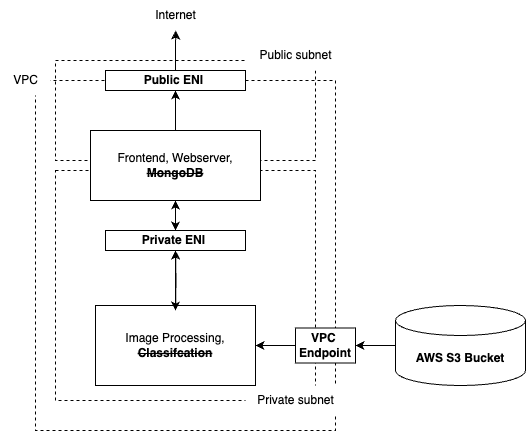
\includegraphics[height=0.9\textheight,width=0.9\textwidth,keepaspectratio]{images/mm_8-13-system.png}
        \end{column}
    \end{columns}
\end{frame}

\begin{frame}{Image Processing Merging}
    \begin{itemize}
        \item Package Management Issues
        \item Python Versioning and Torch?
    \end{itemize} 
\end{frame}

\begin{frame}{Wrapping Up}
    \begin{itemize}
        \item Revisiting Terraform
        \item Frontend Changes
    \end{itemize} 
\end{frame}
% To create a slide, use the following:
% \begin{frame}{TITLE}
%     BODY
% \end{frame}

% To create a slide with a bullet list, use the following:
% \begin{frame}{TITLE}
%     \begin{itemize}
%         \item ITEM 1
%         \item ITEM 2
%     \end{itemize}    
% \end{frame}

% To create a slide with numbered list, use the following:
% \begin{frame}{TITLE}
%     \begin{enumerate}
%         \item ITEM 1
%         \item ITEM 2
%     \end{enumerate}
% \end{frame}

% To create a slide with a graphic:
% 1. Add the graphic to this folder (named picture.png)
% 2. Use the following:
% \begin{frame}{TITLE}
%     \centering
%     \includegraphics[height=0.7\textheight,width=0.7\textwidth,keepaspectratio]{picture.png}
% \end{frame}

% To create a slide with two columns, use the following:
% \begin{frame}{TITLE}
%     \begin{columns}
%         \begin{column}{0.5\textwidth}
%             COLUMN 1 BODY
%         \end{column}
%         \begin{column}{0.5\textwidth}
%             COLUMN 2 BODY
%         \end{column}
%     \end{columns}
% \end{frame}
